\documentclass[11pt]{article}
\usepackage[utf8]{inputenc}
\usepackage{algorithm}
\usepackage{graphicx}
\usepackage{mathtools}
\usepackage{amsfonts}
\usepackage{hyperref}
\usepackage{geometry}
\usepackage{multicol}
\usepackage{capt-of}
\usepackage{url}
\usepackage[italian]{babel}
\geometry{a4paper, top=2.5cm, bottom=2.5cm, left=3cm, right=3cm, bindingoffset=5mm}
\usepackage[suftesi]{frontespizio}

\title{Relazione di Laboratorio - Interferometro di Michelson}
\author{Gruppo VE\_2:\\ \\Federico Greco C.M. 969073\\federico.greco2@studenti.unimi.it\\ \\ Nicolò Favagrossa C.M. 969124\\nicolo.favagrossa@studenti.unimi.it\\ \\Daniele Hasou C.M. 967555\\daniele.hasou@studenti.unimi.it \\ \\ Esperimento eseguito da: Nicolò Favagrossa}
\date{\today\\A.A. 2020-2021}

\begin{document}
\maketitle
\tableofcontents
\newpage
\section{Introduzione}
L'interferometro di Michelson è un'apparato sperimentale costruito e messo a punto dal fisico da cui prende il nome nella seconda metà del '800. Questo interferometro è stato protagonista di numerosi e influenti esperimenti tra cui l'esperimento di Michelson e Morley nel 1887 che provò l'inesistenza dell'etere. 

In questo esperimenza le misure da svolgere attraverso l'interferometro di Michelson sono quattro:
\begin{itemize}
    \item la lunghezza d'onda di un fascio di luce monocromatica;
    \item l'indice di rifrazione dell'aria a pressione atmosferica;
    \item la lunghezza di un pacchetto di luce bianca (non monocromatica);
    \item la separazione tra le due righe del doppietto del sodio.
\end{itemize}
L'importanza dell'interferometro di Michelson è anche legata al fatto che utilizzando semplicemente delle misure di tipo macroscopico (il conteggio delle frange e una distanza nell'ordine dei $mm$) si è in grado di misurare una distanza (la lunghezza d'onda) microscopica.

Nell'immagine sottostante si può visualizzare l'interferometro presente in laboratorio.
\begin{figure}[htp!]
\centering
  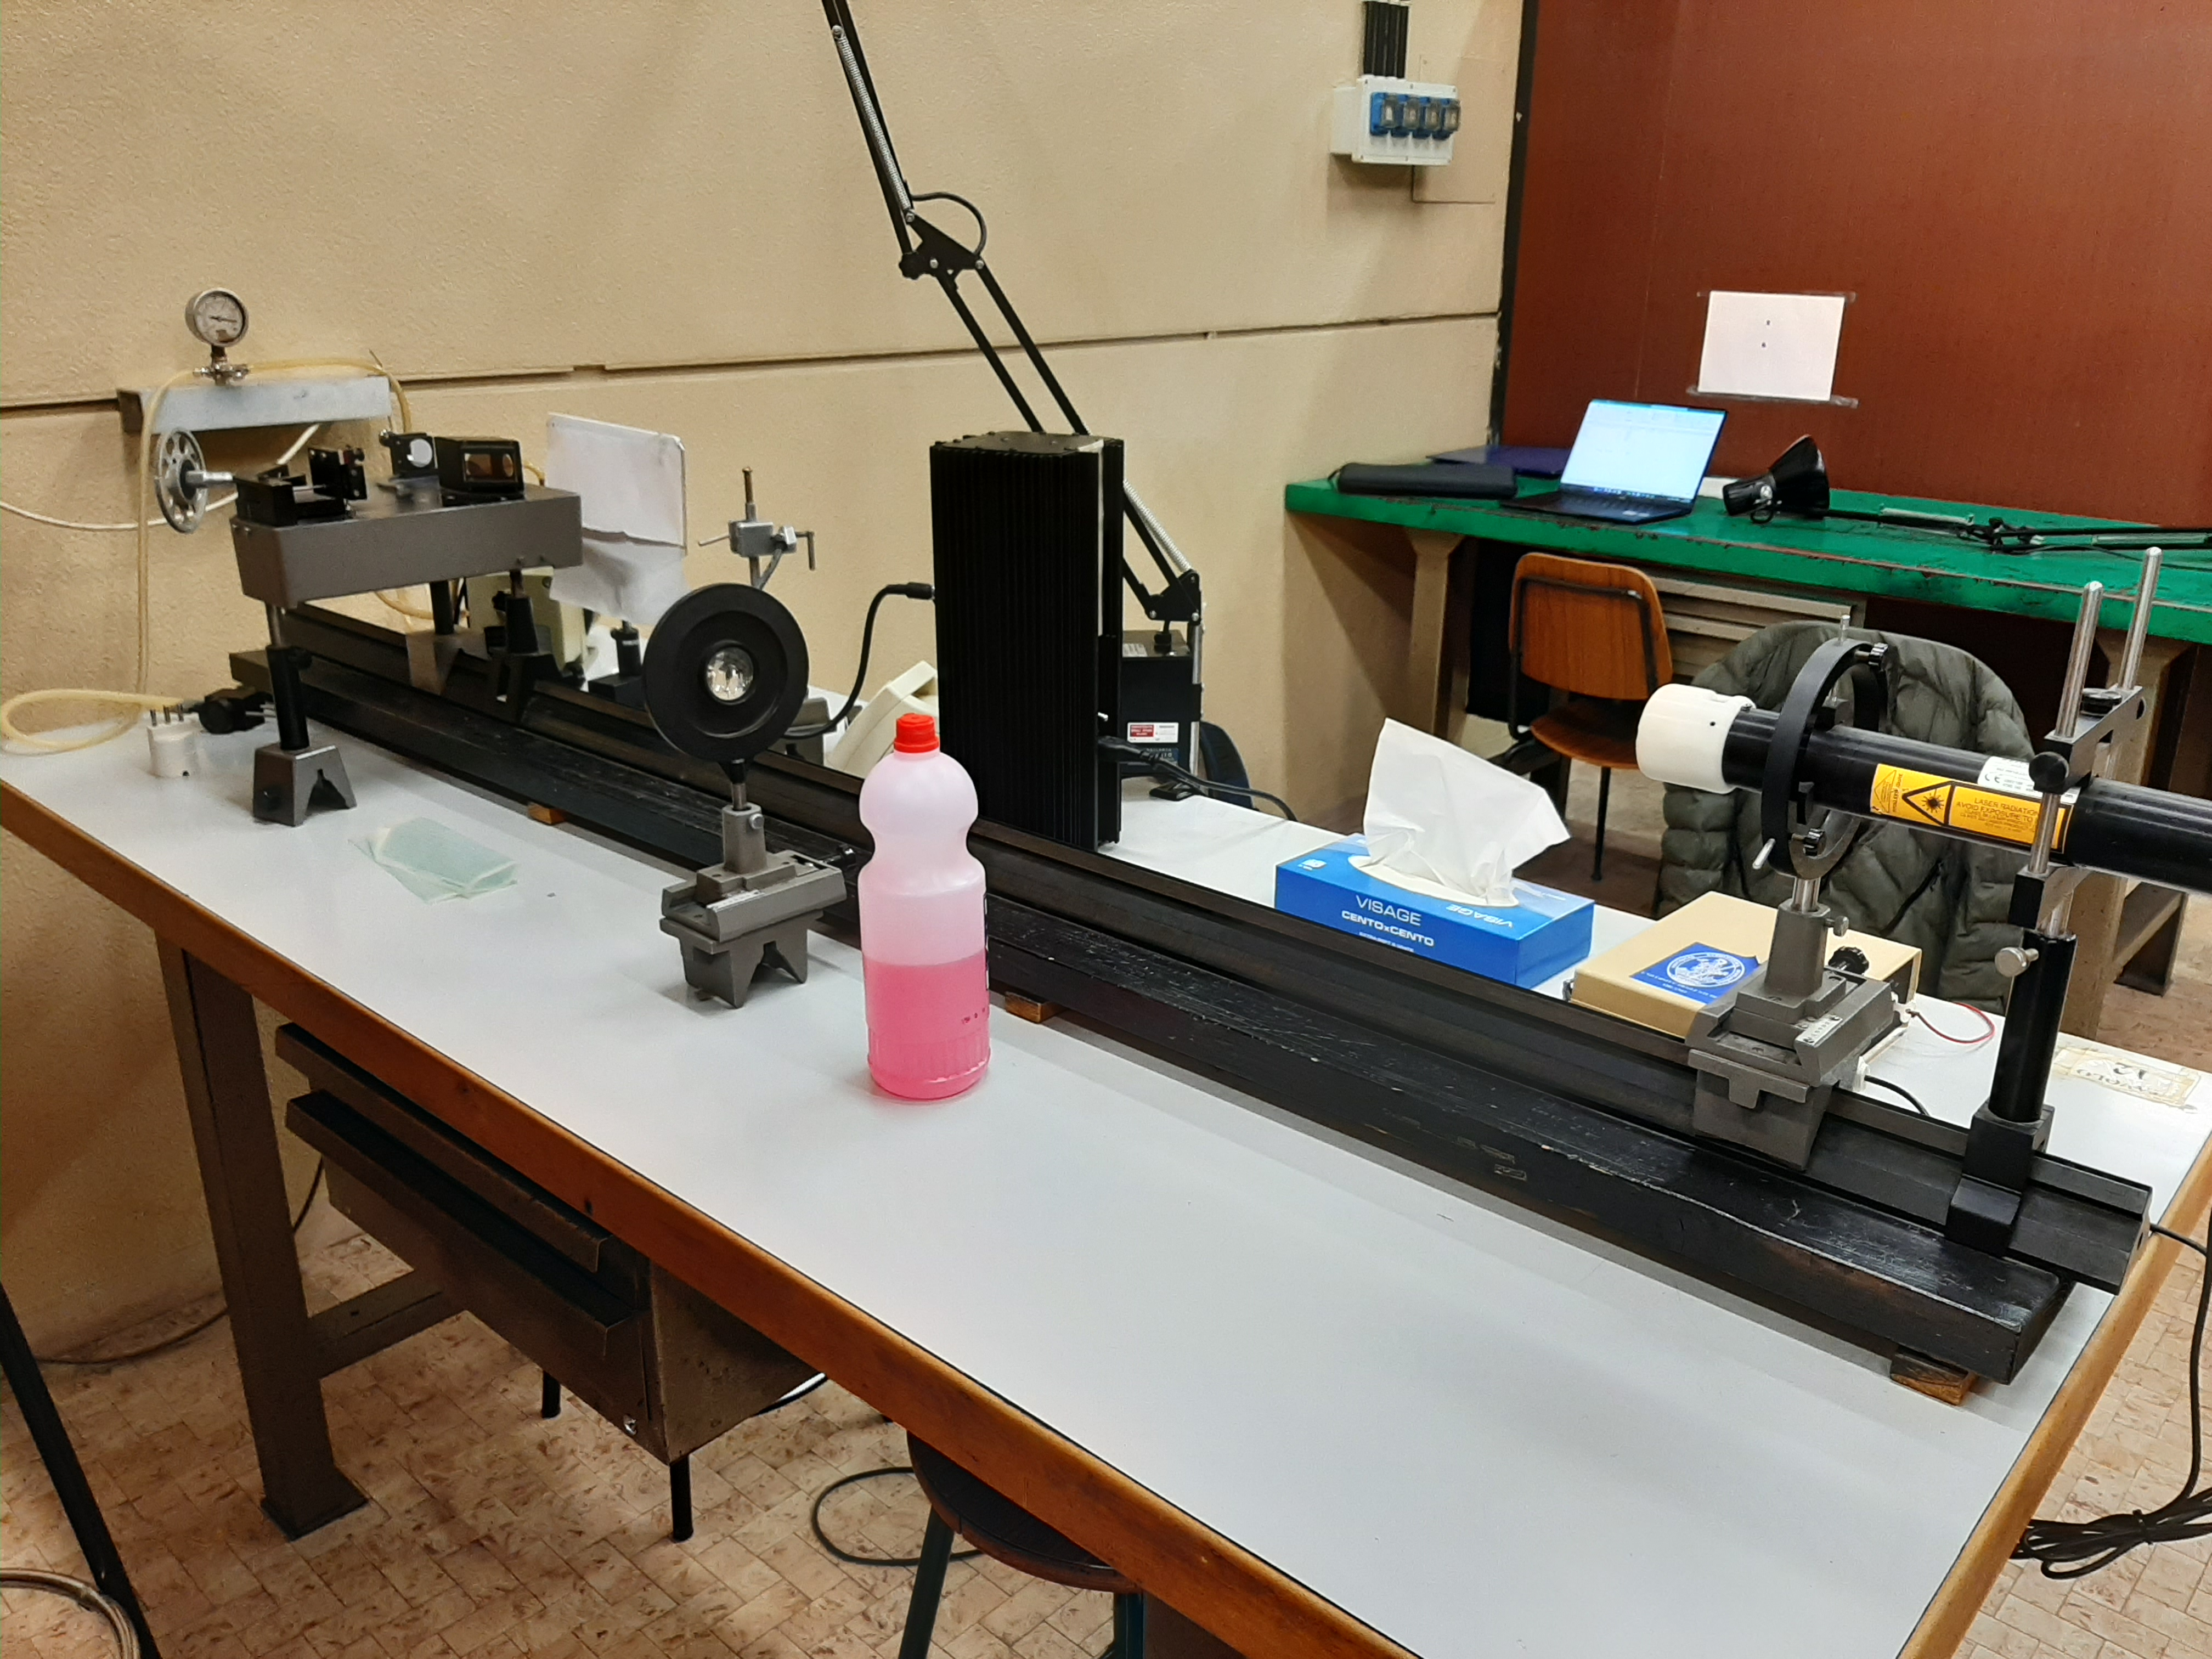
\includegraphics[scale=0.08]{m.jpg}
  \caption{In laboratorio oltre all'interferometro di Michelson (con tutte le sue parti descritte nell'apposita sezione) è presente del materiale per disinfettare la postazione sia all'inizio che alla fine dell'esperienza.}
  \label{M}
\end{figure}
\newpage
\section{Trattazione teorica}
\subsection{Onda elettromagnetica ed interferenza costruttiva e distruttiva}
La luce prodotta da un laser può essere idealizzata come un'onda sinusoidale di frequenza costante e durata infinita. Quest'onda può essere rappresentata dal campo elettrico e dal campo magnetico, ortogonali fra loro ed entrambi in fase ed ortogonali alla direzione di propagazione $\Vec{r}$:
\begin{equation}\begin{split}
    \Vec{E}(\Vec{r}, t) = \Vec{E_0}cos(\Vec{k}\cdot \Vec{r}-\omega t) \\
    \Vec{B}(\Vec{r}, t) = \Vec{B_0}cos(\Vec{k}\cdot \Vec{r}-\omega t)
\end{split}\end{equation}
Dove $\Vec{k}$ è il vettore d'onda, $\Vec{r}$ è il vettore spostamento, $t$ il tempo ed infine $\omega$ è la pulsazione che dipende dal periodo.

Se ci limitiamo a studiare il caso monodimensionale il comportamento dell'onda se si propaga nel vuoto può essere quindi descritto attraverso la seguente equazione:
\begin{equation}
    \psi(r, t) = cos(kr-\omega t)=cos(\frac{2\pi}{\lambda}(r-ct))
\end{equation}
O in un mezzo con indice di rifrazione $n$:
\begin{equation}
    \psi(r, t) = cos(kr-\omega t)= cos(\frac{2\pi}{\lambda_0}(nr-ct))
\end{equation}
dove $nr$ rappresenta il cammino e la lunghezza d'onda nel mezzo è: $\lambda = \frac{\lambda_0}{n}$.

Considerando due onde monocromatiche che abbiano uguale frequenza, se si sovrappongono in un punto P vale che l'intensità è: 
\begin{equation}
    I = I_1 + I_2 +2\sqrt{I_1 I_2}\, cos(\Delta\phi)
\end{equation}
In cui $\Delta\phi = \frac{2\pi}{\lambda_0}(n_1r_1-n_2r_2)$ rappresenta la differenza di fase delle due onde nel punto. Infatti si hanno due condizioni:
\begin{itemize}
    \item $\Delta\phi = 0$ interferenza costruttiva;
    \item $\Delta\phi = \pi$ interferenza distruttiva
\end{itemize}
Se $I_1 \approx I_2 \approx I_0$ l'intensità varierà da $0$ a $4I_0$. 

In laboratorio sono state utilizzate tre diverse sorgenti luminose che si differenziano per il fatto di avere una lunghezza di coerenza più o meno grande. L'approssimazione fatta per un'onda elettromagnetica sinusoidale monocromatica include il fatto che il tempo di emissione di questa onda, quindi il meccanismo fisico che genera quest'onda, ha un tempo di emissione infinito perchè è in grado di mantenere questa sinusoide per un tempo infinito. Questa approssimazione è ottima quando si parla di laser. Usando invece una fonte come una lampada a luce bianca o una lampada al sodio porta ad avere un tempo di emisssione finito $\Delta t$ e quindi l'onda risulta troncata portando alla formazione di pacchetti d'onda di lunghezza $\Delta L$ detta lunghezza di coerenza. Si dimostra che tale pacchetto si ottiene come sovrapposizione di tante onde monocromatiche con frequenza e lunghezza d'onda diverse. Infatti se il tempo di coerenza è molto piccolo, il pacchetto d'onda conterrà molte lunghezze d'onda. Mentre, ad esempio nel laser, $\Delta t$ è molto grande di conseguenza saranno pochissime le lunghezze d'onda presenti nel pacchetto d'onda. Si può scrivere che $\Delta t \Delta \nu \approx 1$.
Per quanto riguarda il laser, avendo un tempo di coerenza infinito non ci saranno problemi nel visualizzare l'interferenza nell'intererometro di Michelson; mentre per la luce bianca c'è interferenza solo entro il tempo di coerenza della sorgente stessa.
\subsection{L'interferometro di Michelson}
L'interferometro di Michelson, illustrato schematicamente nella figura (\ref{Interferometro di Michelson}), è stato utilizzato in laboratario per studiare l'interferenza di due onde coerenti tra di loro. Quindi il modo migliore per assicurare l'interferenza è sdoppiare un'unica sorgente, in questo modo le onde risultanti saranno coerenti. Quindi l'interferometro è un sistemi di specchi che sdoppia il fascio di luce in due cammini differenti.

L'apparato sperimentale è dunque composto in primo luogo da una sorgente, ad esempio un laser o una qualsiasi fonte di luce posizionato su una guida metallica. L'onda elettromagnetica che parte dalla sorgente incontra una lente divergente che serve a rendere l'immagine finale sullo schermo più grande e quindi visibile.

Come mostrato in figura, il fascio di luce incontra una lastra semi riflettente, denominata in figura con $S_1$, posta con un'inclinazione di $45^\circ$ rispetto alla direzione del fascio di luce. La lastra $S_1$ è detta semi riflettente perchè ha una superficie riflettente e l'altra lo è in parte. Infatti quando il fascio di luce incide $S_1$ viene in parte trasmesso e in parte riflesso. La parte riflessa va verso lo specchio piano $S_3$ e viene completamente riflessa, tornando indietro e  riattraversando $S_1$ e successivamente viene trasmesso verso lo schermo.
Contemporaneamente, tornando alla prima incidenza dell'onda elettromagnetica con $S_1$, il fascio di luce trasmesso dalla lastra $S_1$ attraversa una lamina di compensazione $L_c$, incontra lo specchio $S_2$ che riflette completamente il fascio di luce facendolo tornare verso lo specchio $S_1$ in cui viene nuovamente riflesso verso lo schermo. Quindi, alla fine, sullo schermo arrivano due fasci di luce generati da un'unica sorgente che hanno compiuto due cammini differenti.
La lamina di compensazione $L_c$ serve perchè il raggio che va verso $S_3$ ha attraversato $S_1$ tre volte; mentre il fascio di luce che va verso $S_2$ attraversa $S_1$ solo una volta. Quindi se pongo una lamina con lo stesso materiale, spessore e inclinazione di $S_1$ nel cammino che compie il fascio di luce trasmesso da $S_1$ eguaglio il cammino ottico tra i due raggi. 

Tutto il sistema ottico produce due immagini virtuali puntiformi visualizzabili sullo schermo. Le due immagini virtuali si incontrano in fase (o in opposizione di fase) e in cui si avrà una situazione di intensità massima (o minima).

Gli spostamenti di $S_3$ sono effettuati con una vite micrometrica sensibile al centesimo di mm e ridotto di $\frac{1}{5}$ da una leva, portando la sensibilità dello strumento a $2\, \mu m$. Lo specchio $S_2$ ha invece due manopole per inclinarlo nelle due direzioni ed in base alla misura da fare consente di imporre l'ortogonalità. 
\begin{figure}[htp!]
\centering
  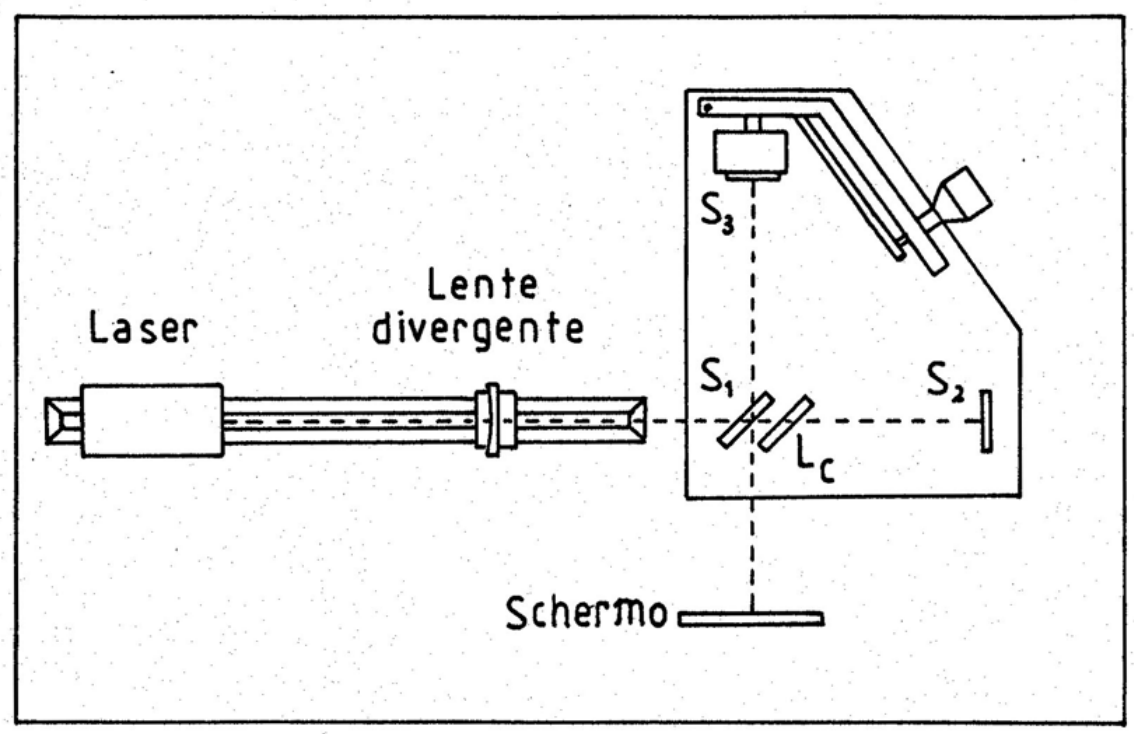
\includegraphics[scale=0.4]{Interferometro di Michelson.png}
  \caption{Nella seguente immagine è illustrato un semplice schema con visuale dall'alto dell'interferometro di Michelson.}
  \label{Interferometro di Michelson}
\end{figure}


Tutto il sistema ottico produce due immagini virtuali puntiformi: $F_1$ e $F_2$. Possiamo quindi dire che al posto dello specchio $S_2$, posizioniamo uno specchio fittizio $S'_2$ parallelo ad $S_3$ ad una sistanza $d$ dallo schermo. La distanza $d$ non è altro che la distanza tra $S_2$ ed $S_1$. Lo specchio virtuale $S'_2$ produce l'immagine virtuale $F_1$ Inoltre si può schematizzare $S_3$ con un'immagine virtuale che si denota con $F_2$, quest'ultima è il fascio di luce che riceve lo schermo dalla riflessione su $S_3$. Attraverso la figura (\ref{Schema}) è possibile visualizzare schematicamente ciò che è stato appena illustrato. 
 Di conseguenza lo sperimentatore vedrà delle figure di interferenza costruttiva quando i due fasci di luce si incontrano in fase, e quindi si avrà la situazione di intensità massima ($I=4I_0$); quando invece si incontrano in opposizione di fase si avrà intensità minima ($I=0$). La differenza di fase dipende quindi dalla differenza di cammino ottico.

\begin{figure}[htp!]
\centering
  
\includegraphics[scale=0.5]{Schema.png}
  \caption{Si può osservare come le immagini virtuali $F_1$ e $F_2$ possano essere sostituite dal sistema di specchi per visualizzare in modo immediato ciò che riceve lo schermo. Dove $d$ rappresenta la distanza tra lo specchio $S_2$ e lo specchio $S_1$.}
  \label{Schema}
\end{figure}
\newpage
\section{Procedura sperimentale - Analisi dati}
In laboratorio è stato necessario prepararsi in precedenza un foglio di calcolo Excel per determinare in modo semplicemente qualitativo la consistenza delle misure fatte. Dopo aver disinfettato il banco di lavoro con fazzoletti e alcol etilico denaturato messo a disposizione dai responsabili del laboratorio si può iniziare a preparare il setup sperimentale.

Prima di iniziare con le quattro diverse misure ci sono alcuni aggiustamenti preliminari. Per prima cosa bisogna imporre una condizione di ortogonalità tra $S_1$ ed $S_2$ con la luce laser, infatti, agendo sulle viti di $S_2$ si fa in modo che i fasci provenienti da $S_3$ e da $S_2$ si sovrappongano sullo schermo. Agendo sulle viti di $S_2$ è possibile modificare l'inclinazione dello specchio in modo tale da allineare i due punti luminosi sullo schermo. Successivamente bisogna inserire sulla guida metallica la lente divergente in modo tale da rendere l'immagine sullo schermo di dimensioni maggiori. Dopo questi aggiustamenti preliminari si dovrebbero vedere le frange di interferenza.
\subsection{Misura della lunghezza d'onda della luce laser}
La prima misura da effettuare in laboratorio è la lunghezza d'onda della luce laser. Dopo aver svolto tutti gli aggiustamenti preliminari è possibile osservare le frange di interferenza sullo schermo. L'esperienza consiste nel scegliere un punto $P$ sullo schermo segnandolo con una matita. Successivamente spostando lo specchio mobile $S_3$ di $\Delta x$ attraverso una vite micrometrica varia il cammino ottico e si osservano le frange di interferenza costruttive chiare (o distruttive scure) che passano per il punto $P$, come si può osservare nell'imamgine (\ref{g}). Contando le frange e misurando la posizione iniziale e finale della vite micrometrica si hanno tutte le misure per ricavare $\lambda$.
Infatti sullo schermo si può osservare un passaggio da un massimo di interferenza al successivo quando si sposta la distanza tra le due sorgenti immagine di una lunghezza d'onda. Questo corrisponde ad aver spostato lo specchio $S_3$ di mezza lunghezza d'onda perchè lo spostamento viene percorso due volte. Se si osserva il passaggio di $N$ frange si ottiene:
\begin{equation}
    2n\Delta x = N \lambda\, \Longrightarrow \,\lambda = \frac{2 n \Delta x}{N}
    \label{formula}
\end{equation}
dove $n$ rappresenta l'indice di rifrazione dell'aria che per questa misura si approssima ad $n = 1$.

Per misurare $\Delta x$ in modo efficiente bisogna assicurarsi di misurare la posizione iniziale e finale in condizioni in cui la lettura della vite micrometrica non sia ambigua. Per quanto riguarda il numero di frange da contare $N$, per rendere l'errore associato a questo conteggio trascurabile rispetto all'errore strumentale è necessario contare più di $130$ frange. Attraverso lo specchio $S_2$ si poteva invece aumentare o diminuire le dimensione delle frange per agevolare la presa dati.

Di seguito allego la tabella che contiene i dati raccolti durante la prima esperienza:
\begin{table}[H]
    \centering
    \begin{tabular}{|c|c|c|}
    \hline
     Numero frange:  & $\Delta x\pm \sigma_{\Delta x} [mm]$ & $ \lambda \pm \sigma_\lambda  [nm]$\\
    \hline
    $150$ & $0.046 \pm 0.003$ & $613.333 \pm 37.712$ \\
    \hline
    $180$ & $0.056 \pm 0.003$ & $622.222 \pm 31.427$ \\
    \hline
    $153$ & $0.048\pm 0.003$ & $627.451 \pm 36.973$ \\
    \hline
    $150$ & $0.046\pm 0.003$ & $613.333 \pm 37.712$ \\
    \hline
    $140$ & $0.044\pm 0.003$ & $628.571 \pm 40.406$ \\
    \hline
    $133$ & $0.042\pm 0.003$ & $631.578 \pm 42.533$ \\
    \hline
    \end{tabular}
    \caption{In questa tabella sono riportate le misure non scartate effettuate in laboratorio con le relative incertezze.}
    \label{L'unghezza d'onda}
\end{table}
L'incertezza relativa allo spostamento $\Delta x$ è stata ricavata attraverso la propagazione degli errori in quanto l'incertezza di una singola misura attraverso la vite micrometrica è di $\sigma_x = 2 \mu m$ di conseguenza: 
\begin{equation}
 \sigma_{\Delta x}= \sqrt{\sigma_x ^2 + \sigma_x ^2}
 \label{posizione}
\end{equation}
e di conseguenza, sempre adottando la propagazione degli errori:
\begin{equation}
    \sigma_\lambda = \frac{2\sigma_{\Delta x}}{N}
\end{equation}
Per stimare il miglior valore tra le misure effettuate ho effettuato la media pesata:
\begin{equation}
    \lambda_{spe}=\frac{\sum_{i} w_i \lambda_i }{\sum_{i} w_i} \qquad w_i= \frac{1}{\sigma_{\lambda}^2}
    \label{media}
\end{equation}
con incertezza relativa
\begin{equation}
    \sigma_{\lambda}=\left(\sum_{1} w_i \right)^{-1/2}
    \label{peso}
\end{equation}
ottendendo:
\begin{equation}
    \nonumber
    \lambda_{spe}= 622 nm \qquad \sigma_\lambda= 15 nm
\end{equation}
Successivamente, ponendo $\lambda_{teo}=633 nm$, attraverso l'osservabile $t$ del test t di Student:
\begin{equation}
    t = \frac{|\lambda_{spe}-\lambda_{teo}|}{\sigma_{\lambda}} 
\end{equation}
Si ricava quindi che $t = 0.28$; dopo aver consultato le tabelle appropriate si ricava la probabilità che la misura sia diversa dal valore teorico per fluttuazioni statische è del $78\%$. Di seguito riporto il grafico in cui si possono visualizzare i valori con le relative barre d'incertezza. Alla luce di questi risultati le due misure sono consistenti.
\begin{figure}[htp!]
\centering
  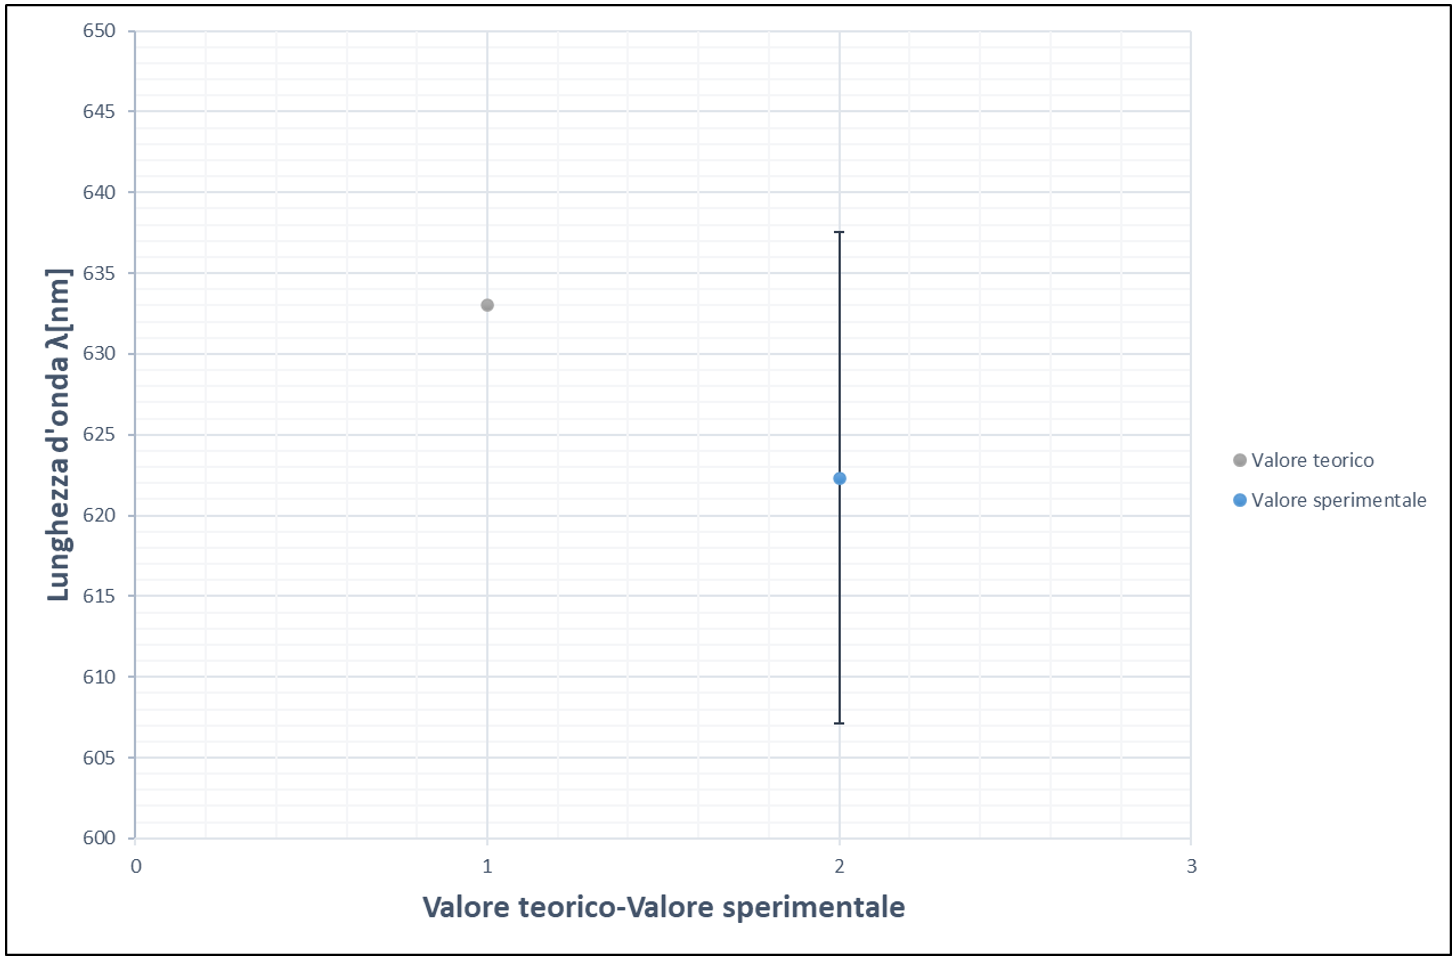
\includegraphics[scale=0.25]{Grafico.png}
  \caption{Nel seguente grafico è possibile visualizzare il confronto tra il valore teorico posto a $633 nm$ e il valore sperimentale che equivale ad $622 nm$ con le barre d'errore che rappresentano l'incertezza della misura che equivale ad $15 nm$}
  \label{gg}
\end{figure}

Durante questa presa dati ho riscontrato qualche difficoltà legata alla vite micrometrica in quando bastava un tremore di mano per perdere completamente la posizione della frangia che si stava contando, a quel punto bisognava ricominciare e iniziare una nuova misura.
\newpage
\subsection{Misura dell'indice di rifrazione dell'aria a pressione atmosferica}
Nella precedente misura si è approssimato l'indice di rifrazione dell'aria ad $n=1$, cioè all'indice di rifrazione nel vuoto. In questa presa dati verificheremo se questa approssimazione è origine di un errore non trascurabile e quindi se è necessario implementare opportune correzioni nella presa dati precedente.

In questa misura si utilizza il laser come sorgette ma a differenza dell'esperienza precedente la variazione del cammino ottico non è più originata dal diverso cammino geometrico ma dovuta dalla variazione dell'indice di rifrazione del mezzo di propagazione. Infatti si inserisce, attraverso una guida apposita, tra lo specchio $S_1$ e $S_2$ una camera cilindrica di lunghezza nota $D=(5.0\pm0.1)cm$. Nella camera cilindrica è possibile creare una situazione approssimabile con il vuoto ($<10^{-1}torr$). 
Di conseguenza la variazione di cammino ottico tra l'aria e l'interno del cilindro è: $2D(n-1)$, quindi se conto $N$ frange di interferenza costruttiva si ottiene:
\begin{equation}
    2D(n-1)=N\lambda_{spe} \quad \Rightarrow \quad n=\frac{N\lambda_{spe}}{2D}+1
    \label{indice}
\end{equation}

Sperimentalmente bisogna inserire la camera cilindrica tra $S_1$ ed $S_2$, la camera è collegata con un tubo in plastica alla pompa per creare il vuoto. Dopo aver acceso la pompa bisogna osservare il manometro fino a quando arriva a fondo scala. Dopo aver spento la pompa, attraverso una valvola, bisogna far rientrare l'aria nella camera in modo da visualizzare e contare il passaggio delle frange dal punto $P$ scelto. Questo procedimento va ripetuto fino a quando non si ottengono almeno cinque o più misure.

Di seguito le misure effettuate in laboratorio:
\begin{table}[H]
    \centering
    \begin{tabular}{|c|c|}
    \hline
     Numero frange:  & Indice di rifrazione $n$  \\
    \hline
    $41$ & $ 1.000255 \pm 8 \times 10^{-6}$  \\
    \hline
    $41$ & $ 1.000255 \pm 8 \times 10^{-6}$  \\
    \hline
    $43$ & $ 1.000268\pm 8 \times 10^{-6}$  \\
    \hline
    $44$ & $ 1.000274\pm 9 \times 10^{-6}$  \\
    \hline
    $42$ & $ 1.000261\pm 8 \times 10^{-6}$  \\
    \hline
    $42$ & $ 1.000261\pm 8 \times 10^{-6}$  \\
    \hline
    \end{tabular}
    \caption{In questa tabella sono riportate le misure non scartate effettuate in laboratorio con le relative incertezze.}
    \label{Indice di rifrazione}
\end{table}
L'incertezza è stata calcolata attraverso la formula di propagazione degli errori
\begin{equation}
    \sigma_n=\sqrt{\left(\frac{N}{2D}\right)^2 \sigma_\lambda^2 + \left(-\frac{N\lambda}{2D^2}\right)^2 \sigma_D^2}
\end{equation}
La migliore stima dell'indice di rifrazione è stato ottenuto attraverso la stessa formula della media ponderata usata nella precedente analisi dati (\ref{peso}) ottenendo come risultato:
\begin{equation}
    \nonumber
    n_{spe}=1.000262 \qquad \sigma_n = 7 \times 10^{-6}
\end{equation}
In conclusione se nella formula (\ref{formula}) non avessi approssimato l'indice di rifrazione il risultato non sarebbe variato sigificativamente in quanto l'errore portato da questa approssimazione è trascurabile rispetto all'errore propagato dello strumento di misura.
\newpage
\subsection{Misura della lunghezza di un pacchetto di luce bianca}
La luce bianca prodotta da una lampada ad incandescenza, come illustrato nella sezione di trattazione teorica, non è una sorgente coerente infatti, a differenza del laser, non emette una sinusoide infinita ma pacchetti d'onda di lunghezza $L$. 

Prima di posizionare la lampada ad incandescenza sulla guida metallica (andando a rimuovere la lente divergente), bisogna rendere il cammino geometrico dei due semi pacchetti provenienti dallo stesso pacchetto approssimativamente uguali. Per farlo si sfrutta una proprietà molto importante dell'interferometro infatti i due specchi $S_2$ ed $S_3$ possono essere ortogonali o non ortogonali tra di loro formando delle frange diverse in situazioni diverse. Quando i due specchi non sono ortogonali fra di loro e la distanza fra le due sorgenti immagine $F_1$ ed $F_2$ è minima si forma delle frange rettilinee.

In laboratorio quindi ho misurato la posizione in cui le frange passano da una forma concava ad una forma rettilinea e ho misurato la posizione di passaggio tra la forma rettilinea e il cambio di concavità. In questo modo ho individuato l'intervallo in cui il braccio dello specchio $S_3$ e approssimativamente uguale al braccio dello specchio $S_2$. Togliendo la lente divergente e oscurando il laser ho posizionato la fibra ottica, collegata alla lampada ad incandescenza, vicino all'interferometro di Michelson ed ho cominciato a cercare delle frange colorate nell'intervallo individuato nella fase precedente. Spostando lentamente lo specchio $S_3$ si cerca quindi la situazione in cui si visualizzano delle frange colorate. Successivamente, una volta individuate le frange colorate, per misurare la lunghezza del pacchetto di luce bianca, con l'ausilio della vite micrometrica, bisogna misurare la posizione di quando si iniziano ad intravedere le frange colorate e il momento in cui svaniscono. In questa maniera con una sottrazione in modulo si ottiene la lunghezza del pacchetto di luce.
\begin{equation}
    L=\Delta x
\end{equation}
Di seguito riporto la tabella con i valori misurati in laboratorio:
\begin{table}[H]
    \centering
    \begin{tabular}{|c|c|c|}
    \hline
     Xiniziale[mm] & Xfinale [mm] & L[mm] \\
    \hline
    $15.89$ & $15.86$ & $0.006$ \\
    \hline
    $15.89$ & $15.85$ & $0.008$ \\
    \hline
    $15.89$ & $15.85$ & $0.008$ \\
    \hline
    $15.85$ & $15.89$ & $0.008$ \\
    \hline
    $15.85$ & $15.89$ & $0.008$ \\
    \hline
    \end{tabular}
    \caption{In questa tabella sono riportate le misure non scartate effettuate in laboratorio con le relative incertezze.}
    \label{pacchetto}
\end{table}
Facendo la media e attraverso la propagazione degli errori (\ref{posizione}) si ottiene:
\begin{equation}
    \nonumber
    L_{spe}=7.6\mu m \qquad \sigma_L=2.8 \mu m
\end{equation}
\subsection{Misura della separazione tra le due righe del doppietto del sodio}
In quest'ultima misura si utilizza una lampada ai vapori di $Na$ (sodio) che emette due particolari l'unghezze d'onda gialle, $\lambda_1=5890$\r{A} e $\lambda_2=5896$\r{A}, di intensità simile e separazione piccola rispetto alla $\lambda$ media infatti distano di $6$\r{A}. La lampada al sodio si colloca in una situazione intermedia tra la lunghezza di coerenza del laser e della lampada a luce bianca ad incandescenza, infatti la lunghezza di coerenza della lampada al sodio e di qualche centimetro.

In laboratorio si possono osservare delle frange nitide quando le due lunghezze d'onda interferiscono in modo tale che le frange chiare della prima lunghezza d'onda si sovrappongono alle frange chiare della seconda l'unghezza d'onda e così anche per le frange scure. Spostando lo specchio $S_3$ di una certa distanza $\Delta x$ si osserva che le frange non sono più visibili e si è in una situazione di luce diffusa. Definendo il numero $m$ le volte in cui si osserva l'alternanza tra figure di interferenza nette, luminosità omogenea e la successiva apparizione delle frange. In questo modo attraverso alcuni conti si ricava la seguente relazione:
\begin{equation}
    \Delta \lambda = \frac{m\lambda^2}{2\Delta x} \qquad m\ge3
\end{equation}
Dove $\lambda=5893$\r{A} è il valore medio tra $\lambda_1$ e $\lambda_2$. Misurando quindi la posizione iniziale, il numero di volte in cui appaiono le frange nitide e la posizone finale sono in grado di misurare, in maniera indiretta, la distanza tra le due lunghezze d'onda.

Di seguito riporto una tabella con le misure svolte in laboratorio:
\begin{table}[H]
    \centering
    \begin{tabular}{|c|c|c|}
    \hline
     m & $\Delta x [mm]$ & $\Delta \lambda \pm \sigma_{\Delta \lambda}$ [\r{A}] \\
    \hline
    $4$ & $1.15$ & $6.04 \pm 0.01$ \\
    \hline
    $4$ & $1.14$ & $6.09 \pm 0.02$ \\
    \hline
    $3$ & $0.85$ & $6.13 \pm 0.02$ \\
    \hline
    $3$ & $0.82$ & $6.32 \pm 0.02$ \\
    \hline
    $3$ & $0.85$ & $6.13 \pm 0.02$ \\
    \hline
    \end{tabular}
    \caption{In questa tabella sono riportate le misure non scartate effettuate in laboratorio con le relative incertezze.}
    \label{distanza}
\end{table}
Per calcolare l'incertezza relativa alla singola misura si è svolta la propagazione degli errori:
\begin{equation}
    \sigma_{\Delta \lambda} = \frac{m\lambda^2}{2\Delta x^2}\sigma_{\Delta x}
\end{equation}
Svolgendo la media e calcolando la deviazione standard si ottiene:
\begin{equation}
    \nonumber
    \Delta \lambda_{spe}= 6.12 \text{\r{A}} \qquad \sigma_{\Delta \lambda} = 0.11
\end{equation}
\begin{figure}[htp!]
\centering
  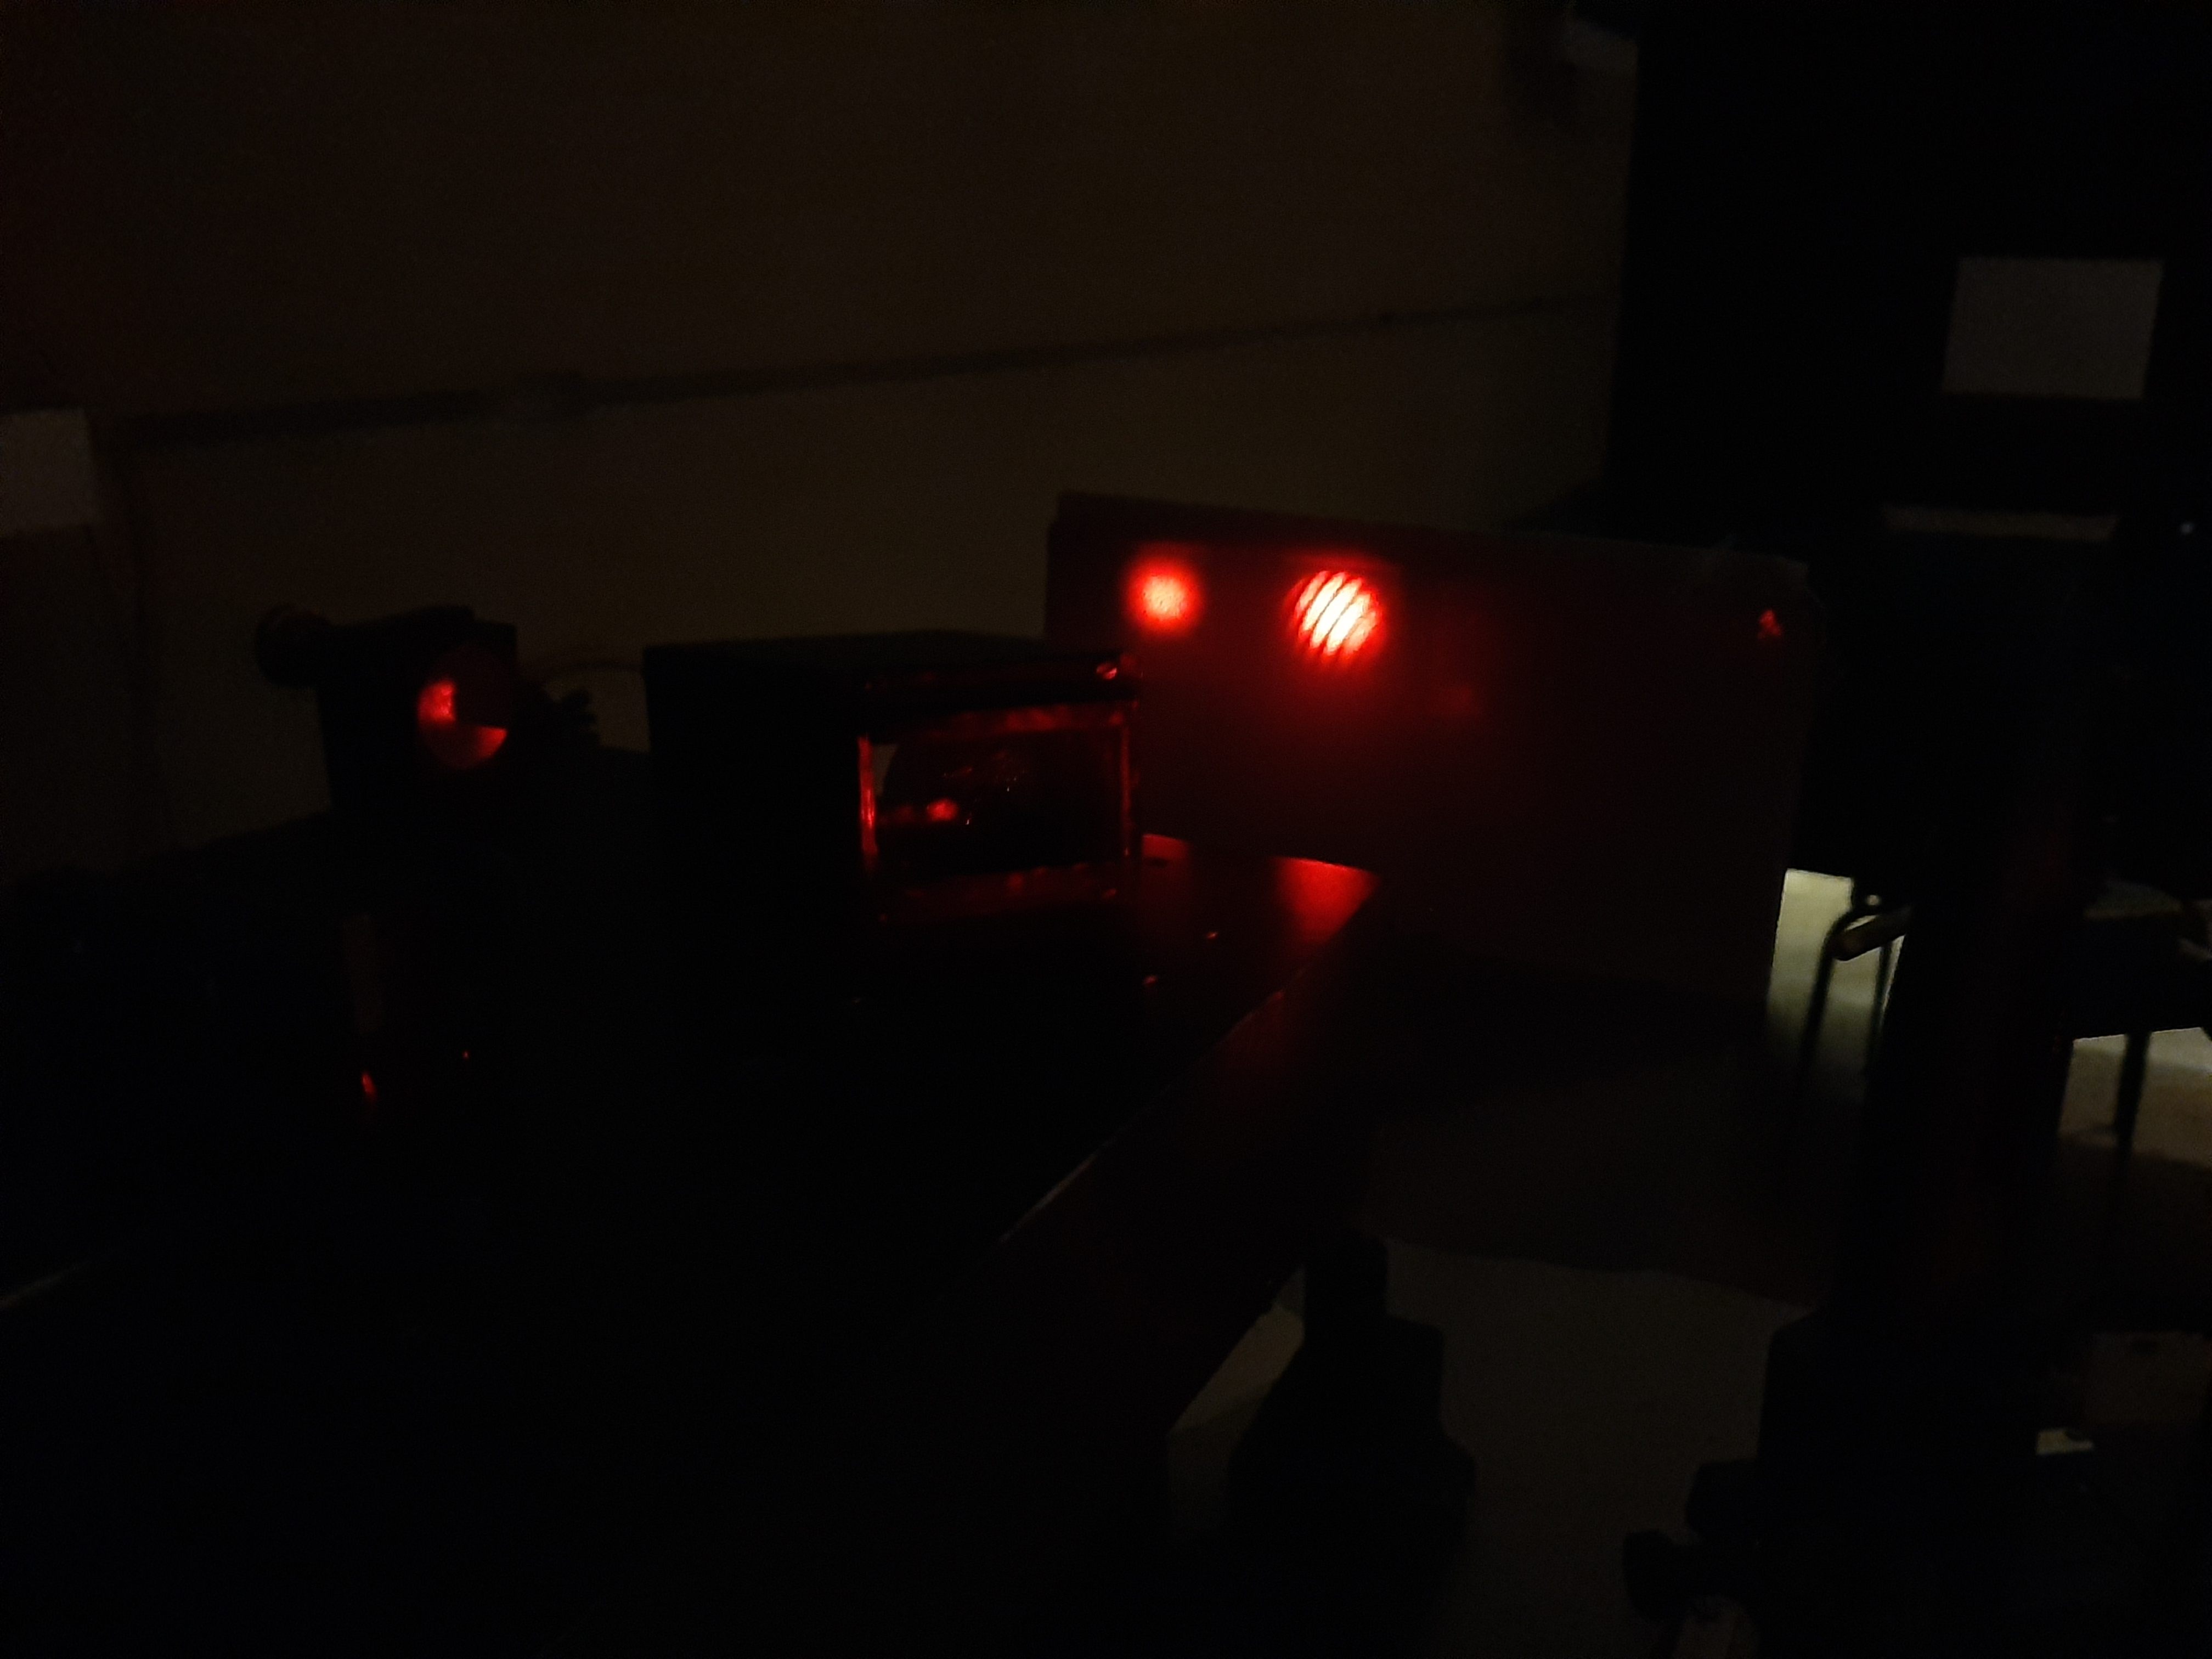
\includegraphics[scale=0.05]{g.jpg}
  \caption{In questa immagine si possono visualizzare le frange chiare e le frange scure durante la misura della lunghezza d'onda del fascio di luce monocromatica.}
  \label{g}
\end{figure}
\section{Conclusione}
Ricapitolando gli obbiettivi dell'esperienza sono: utilizzando l'interferometro di Michelson misurare la lunghezza d'onda di un fascio di luce monocromatica, misurare l'indice di rifrazione dell'aria a pressione atmosferica, la lunghezza di un pacchetto di luce bianca (non monocromatica) ed infine misurare la separazione tra le due righe del doppietto del sodio.

La lunghezza d'onda del laser rosso che è stata misurata è: $\lambda_{spe}=(622\pm15)\,nm$ ed attraverso il test t di Student si ottiene che il valore sperimentale è compatibile con il valore teorico per il $78\%$ di probabilità. Successivamente, per misurare l'indice di rifrazione dell'aria abbiamo utilizzato il valore misurato in precedenza ottenendo: $n_{spe}=1.000262\pm7\times10^{-6}$ solo qualitativamente compatibile con il valore teorico in condizioni standard\footnote{Per condizioni standard si intende a temperatura e pressione standardizzata: $T=0\,\text{°C}$, $P=1\, bar$}. Per la seconda metà dell'esperienza, si è studiata la lunghezza di coerenza di una fonte di luce non monocromatica e con un tempo di coerenza finito, misurando: $L_{spe}=(7.1\pm2.8)\,\mu m$. Infine utilizzando una luce ai vapori di sodio si è verificata la distanza tra due diverse lunghezze d'onda gialle caratteristiche di questo elemento. Dopo 5 misure e l'analisi dati abbiamo ottenuto: $\Delta\lambda_{spe}=(6.12\pm0.11)\, \text{\r{A}}$. Durante l'esperienza sono stati raggiunti tutti gli obiettivi.

\end{document}
